\chapter{Nonlinear Perturbations}

\section{Approaches for non-linear structure formation}

Remember that at late times, perturbations become non-linear ($\delta > 1$), and that according to the Hiearchical structure formation small-scale perturbations become non-linear first.
Perturbations collapse to form dark halos, filaments, and pancakes.
This structure is called the cosmic web, which is a signature of non-linear gravitational instability in an expanding universe.
% movie (illustris collaboration)

Studying the evolution of non-linear perturbations is very difficult, and no exact analytic solutions have yet been found in the fully non-linear regime.
There are different approaches to tackle the problem:
\begin{itemize}
	\item Numerical simulations: They give accurate results, but they are resource-intensive and give less insight than a (hypothetical) fully analytical approach.
	\item Higher order perturbation theory: This is only a valid approach for mildly non-linear perturbations and scales.
	In particular, it is not a good approach for small-scale structures.
	\item Simplified models, in e.g. the Halo model: This is a very successful model in describing the formation, evolution, and statistics of collapsed (non-linear) structures.
% >>>>>>> 606bc2ca57c4ed6f1a9ba40631c6823f0f8a9ba5
\end{itemize}

We will study mainly the Halo model. We start with a model that only contains dark matter, and later introduce baryons.

\section{Spherical Collapse}

We consider a spherical overdensity within an otherwise homogeneous expanding universe. Outside the sphere, the density is $\bar{\rho}$, while inside it is $\rho = \bar{\rho}(1+\delta)$.

We make a few simplifying assumptions:
\begin{itemize}
	\item The universe is flat and matter-dominated, such that $\Omega_0 = \Omega_{\text{m}, 0} = 1$.
	\item There is only collisionless dark matter.
\end{itemize}
We now look at a thin shell with radius $r$ inside the top-hat sphere, and write down its equation of motion. Newton's second law states
\begin{align*}
	\dv[2]{r}{t}
	&= - \frac{G M}{r^2},
\end{align*}
where $M$ is the mass inside the radius $r$,
\begin{align*}
	M = M(r) = \frac{4\pi r^3}{3} \bar{\rho}(1+\delta).
\end{align*}
Note that $M(r)$ is constant as long as the different shells don't cross each other, which we assume for now. 
If we integrate Newton's second law, we get the energy per unit mass of the shell, also called its specific energy $\epsilon$, which is the sum of a kinetic and a potential term:
\begin{align*}
	\epsilon = \frac{1}{2} \left( \dv{r}{t} \right)^2
	- \frac{G M}{r},
\end{align*}
The specific energy is constant because of conservation of energy.
If $\epsilon \geq 0$, the shell expands forever, and if $\epsilon < 0$, the shell first expands, but then it eventually contracts and collapses. We will focus on the latter case.

The solution of the equation of motion for $\epsilon < 0$ is
\begin{align*}
	r &= A(1- \cos \theta) &
	t &= B(\theta - \sin\theta) &
	A &= \frac{GM}{2 \abs{\epsilon}} &
	B &= \frac{GM}{(2 \abs{\epsilon})^{3/2}}
\end{align*}
The solution $r(t)$ is plotted in \cref{fig:shell-collapse-r}.
The shell expands, reaches a maximum radius $r_\text{ta} = 2 A$ at $t_\text{ta} = \pi B$, and collapses at $t_\text{coll} = 2 t_\text{ta}$.\sidenote{We will show that $t_\text{coll} = 2 t_\text{ta}$ in \cref{ssec:virial-applications}, but we have to derive the Virial theorem first.}
However, the model will be invalid shortly before $t_\text{coll}$, since shells start crossing and virialize, which will be discussed later.
\begin{figure}
	\centering
	\import{img/ch-04/}{shell-evolution-r.pdf_tex}
	\caption{The evolution of the shell radius of a spherical overdensity, with negative total energy. The shell expands, reaches a maxium radius, and collapses, which is described by the analytical solution derived in the text. Shortly before collapse, the solution becomes invalid as shells start crossing.}
	\label{fig:shell-collapse-r}
\end{figure}



We would also like to derive an expression for $\rho(t)$ inside the sphere, and find the critical density which is required for collapse. To do this, we use a few more of our assumptions and perform some approximations.

At an early time $t_i$, we define $r=r_i$ and $v = v_i$ as the initial condition. We assume that at $t_i$, the shell follows the Hubble flow:
\begin{align*}
	v_i
	&= \dv{(a x_i)}{t} 
	= \dot{a} x_i &&\text{no peculiar velocity, and } r = a x\\
	&= H r_i.
	&& H = \dot{a}/a 
\end{align*}
Plugging in $t=t_i$, we find
\begin{align*}
	M
	= \frac{4\pi r_i^3}{3}  \bar{\rho}(t_i)(1+\delta_i),
	\qquad
	\epsilon
	= \frac{v_i^2}{2}  - \frac{GM}{r_i}.
\end{align*}
Since we assumed a matter-dominated universe, $a \propto t^{2/3}$ and $H = 2/(3t)$, as well as a flat universe
\begin{align*}
	\bar{\rho}
	= \rho_\text{crit}
	= \frac{1}{6\pi G t^2}.
\end{align*}
We can plug these expressions into the definitions of $A$ and $B$ to get
\begin{align*}
	A = \frac{3}{10} \frac{r_i}{\delta_i},
	\qquad
	B = \frac{9}{20} \frac{t_i}{\delta_i}.
\end{align*}

The density inside the top hat sphere is then
\begin{align*}
	\rho
	&= \frac{M}{\frac{4\pi}{3}r^3}
	= \frac{3M}{4\pi A^3} (1-\cos\theta)^{-3}
	&&\text{because } r = A(1-\cos\theta),
\end{align*}
while outside it is
\begin{align*}
	\bar{\rho}
	&= \frac{1}{6\pi G t^2}
	= \frac{1}{6 \pi G B^2} (\theta-\sin\theta)^{-2}
	&& \text{because } t = B(\theta - \sin\theta).
\end{align*}
It follows that
\begin{align*}
	1 + \delta
	= \frac{\rho}{\bar{\rho}}
	= \frac{9}{2} \frac{(\theta-\sin\theta)^{2}}{(1-\cos\theta)^3}.
\end{align*}
Since we want to find $\rho(t)$ instead of $\rho(\theta)$, we have a little more work to do.
An analytical solution is nowhere to be seen, so we try to find at least an approximation.
At early times, $t << t_\text{ta}$, we perform a Taylor expansion in $t$ and $\theta$ to get
\begin{align*}
	\delta \approx \frac{3}{20} \theta^2
	\qquad
	t \approx \frac{B}{6} \theta^3.
\end{align*}
These two expressions can be combined to find
\begin{align*}
	\delta
	= \frac{3}{20} \left( \frac{6 t}{B} \right)^{2/3}
	= \frac{3}{20} (6\pi)^{2/3} \left( \frac{t}{t_\text{ta}} \right)^{2/3},
\end{align*}
which is fortunately\sidenote{Since we assumed early times, linear perturbation theory should still be valid, so comparing our new result to what we found in the previous chapter gives us some reassurance that everything still works correctly.} in agreement with what we found in linear perturbation theory for a matter-dominated universe, where we derived $D(z) \propto a \propto t^{2/3}$.
Note that this result is only valid at early times, and the actual value of $\delta$ might be quite different at later times. To make things clearer, we define
\begin{align*}
	\delta_\text{lin} = \frac{3}{20} (6\pi)^{2/3} \left( \frac{t}{t_\text{ta}} \right)^{2/3},
\end{align*}
and expect $\delta = \delta_\text{lin}$ at early times, but not at late times. We can find $\rho$ from $\delta$, and $\rho_\text{lin}$ from $\delta_\text{lin}$, which is a more intuitive value. The relationship between $\rho$, $\rho_\text{lin}$, and the density outside the sphere, $\bar{\rho}$, is shown in \cref{fig:shell-collapse-rho}.

\begin{figure}
	\centering
	\import{img/ch-04/}{shell-evolution-rho.pdf_tex}
	\caption{The evolution of the density of a spherical overdensity with negative total energy. The exact model is $\rho$, which agrees well with the linearised approximation $\rho_\text{lin}$ at early times, but only until the turn-around time. For reference, the average density $\bar{\rho}$ of the universe outside the sphere is also shown.}
	\label{fig:shell-collapse-rho}
\end{figure}

The overdensity from the linearized model and the exact model at different times are compared in \cref{tab:exact-vs-lin}.
We notice that the overdensities are larger than one, which in hindsight clarifies why we require non-linear perturbation theory. In the previous chapter, we always assumed $\delta \ll 1$, which is obviously not valid any more.
\begin{margintable}
	\begin{tabular}{lll}
		\toprule
		model & $t_\text{ta}$ & $t_\text{coll}$\\
		\midrule
		$\delta$ & 4.55 & $\infty$\\
		$\delta_\text{lin}$ & 1.062 & 1.686\\
		\bottomrule
	\end{tabular}
	\caption{Overdensities in the linearized and the exact model at different times.}
	\label{tab:exact-vs-lin}
\end{margintable}

Depending on the cosmological models, the overdensity $\delta_c$ required for collapse is different. We have so far worked with a simplified CDM model (sCDM), where we assumed that the universe is flat and dominated by collisionless dark matter. For other cosmologies, such as OCDM and ΛCDM, it turns out that multiplying the sCDM result with an additional factor yields a good approximation:
\begin{align*}
	\delta_c \approx
	\begin{cases}
	1.686 & \text{for sCDM}\\
	1.686 [\Omega_m(t_\text{coll})]^{0.0185} & \text{for OCDM}\\
	1.686 [\Omega_m(t_\text{coll})]^{0.0055} & \text{for ΛCDM}
	\end{cases}
\end{align*}




\section{Collisionless dynamics}

\subsection{Time scales}
\label{ssec:time-scales}

In the previous chapter, we assumed a collisionless medium. To find out when this approximation is valid, we look at the collision time-scales in thermodynamic equilibrium.

We consider a system with $N$ self-gravitating particles and size $r$.
Each particle $i$ has a velocity $\vec{v}_i$ and a mass $m$. The average velocity is $v = \avg{v_i}$.
There are several relevant time scales.
\begin{itemize}
	\item The \emph{crossing time scale} $t_\text{cross}$ is the time required for a typical particle to cross the system:
	\begin{align*}
		t_\text{cross} = \frac{r}{v}
	\end{align*}

	\item The \emph{time scale for direct encounters} $t_\text{direct}$ is the average time a direct encounter of two particles. We find that 
	\begin{align*}
		t_\text{direct}
		=  \left( \frac{r}{r_p} \right) ^2\frac{t_\text{cross}}{N},
	\end{align*}
	where $r_p$ is the particle radius. 
	\item The \emph{time scale for close encounters} $t_\text{close}$ is the average time between close encounters.
	To calculate it, we look at a gravitational two-body interaction of two close particles.
	We define an encounter as a close encounter if the change of the speed of the particle due to the interaction is similar to the initial speed,
	\begin{align*}
		\delta_v
		\defeq \abs*{\vec{v}_\text{before} - \vec{v}_\text{after}}
		\approx \vec{v}_\text{before}.
	\end{align*}
	Then we define $t_\text{close}$ as the average time between close encounters,\sidenote{It seems counter-intuitive that the time between encounters increases with particle size. This has to do with our assumption that the system is in thermodynamic equilibrium, where the velocity goes down for constant $m$ and $r$.}
	\begin{align*}
		t_\text{close}
		= N t_\text{cross}.
	\end{align*}

	\item The \emph{relaxation time scale} $t_\text{relax}$ is the time required for the particle velocity distribution to relax to a new distribution.
	Consider a cumulative change in velocity $\Delta v^2$ over the motion of a particle.
	We define $t_\text{relax}$ as the time scale for which $\Delta v^2$ is comparable to $v^2$. One can show that
	\begin{align*}
		t_\text{relax}
		= \frac{N}{10 \ln N} t_\text{cross}.
	\end{align*}
\end{itemize}

In typical astrophysical systems with $N \gg 100$, such as galaxies and galaxy clusters, we usually find
\begin{align*}
	t_\text{direct} \gg t_\text{close} \gg t_\text{relax} \gg t_H \gg t_\text{cross},
\end{align*}
where $t_H = H^{-1} \approx \SI{e10}{\year}$ is the Hubble time.
Collisions are thus so rare that we can treat many systems as effectively collisionless.

For example, in a galaxy we have $r \approx \SI{10}{\kilo\parsec}$, $v \approx \SI{200}{\kilo\meter\per\second}$, and $N \approx 10^{10}$, which yields
\begin{align*}
	t_\text{direct} &= \SI{e21}{\year},\\
	t_\text{close} &= \SI{5e17}{\year},\\
	t_\text{relax} &= \SI{2e15}{\year},\\
	t_H &= \SI{e10}{\year},\\
	t_\text{cross} &= \SI{5e7}{\year}.
\end{align*}
Gravitational collisions are apparently very inefficient and can be neglected for these systems, so we can use the collisionless Boltzmann equation. Instead of analysing two-body forces, we can use a smooth mean gravitational potential.

\subsection{Basic Dynamics}

The dynamics of the system can be found from the collisionless Boltzmann equation (CBE), with a phase-space distribution function $f(\vec{x}, \vec{v}, t)$.
As we've seen before, the moments of $f$ are
\begin{itemize}
	\item the number density $n(\vec{x}, t) = \int f(\vec{x}, \vec{v}, t) \dd{^3v} = \rho(\vec{x}, t)/m$,
	\item a general moment $\avg{Q}(\vec{x}, t) = \frac{1}{n} \int \dd{^3v} Q f(\vec{x}, \vec{v}, t)$.
\end{itemize}
The evolution of the distribution function is given by the CBE,
\begin{align*}
	\dv{f}{t}
	= \pdv{f}{t} + \sum_i \pdv{f}{x_i} \dv{x_i}{t} + \sum_i \pdv{f}{v_i} \dv{v_i}{t}
	= 0,
\end{align*}
which can be rewritten with $v_i = \dv*{x_i}{t}$ and $\dv*{v_i}{t} = - \pdv*{\Phi}{x_i}$ as
\begin{align*}
	\pdv{f}{t} + \sum_i v_i \pdv{f}{x_i} - \sum_i \pdv{\Phi}{x_i} \pdv{f}{v_i} = 0,
\end{align*}
where the gravitational potential can be calculated from the Poisson equation, $\Lap \Phi = 4 \pi G \rho$.

\subsection{Equations of motion}
\label{ssec:collisionless-eom}

We multiply the CBE by $Q$ and integrate over $\vec{v}$ to get
\begin{align*}
	\pdv{}{t} [n \avg{Q}]
	+ \sum_{i} \pdv{}{x_i}[n \avg{Q v_i}]
	+ n \sum_{i} \pdv{\Phi}{x_i} \avg{ \pdv{Q}{v_i} }
	= 0,
\end{align*}
where the last term follows from partial integration and from $f=0$ for $v^2 \to \infty$.
It turns out that we can completely recover something that looks almost identical to the ideal fluid equations, just by substituting cleverly for $Q$.
\sidenote{We have already seen this in \cref{sec:collisionless-gas}, but we didn't prove the result.}

\paragraph*{Continuity equation}
If we set $Q = 1$, we get
\begin{align*}
	\pdv{n}{t} + \sum_{i} \pdv{}{x_i} [n \avg{v_i}]
	= 0,
\end{align*}
which we recognize as the continuity equation of an ideal fluid, with $n$ instead of $\rho$.

\paragraph*{Euler equation}
For $Q = v_j$, we obtain
\begin{align}
	\label{eq:euler-collisionless}
	\pdv{}{t}[n \avg{v_j}]
	+ \sum_{i} \pdv{}{x_i} [n \avg{v_i v_j}]
	+ n \pdv{\Phi}{x_j}
	= 0.
\end{align}
We remember the definition\sidenote{We have previously defined the stress tensor as $\rho \sigma_{ij}^2$, but we will see the quantity $n \sigma_{ij}^2$ appear now. It does not matter much, because we can convert with $n = \rho/m$.}
\begin{align*}
	\sigma_{ij}^2 = \avg{v_i v_j} - \avg{v_i} \avg{v_j}
\end{align*}
to get
\begin{align*}
	0
	&= \pdv{n}{t} \avg{v_j}
	+ n \pdv{\avg{v_j}}{t}
	+ \sum_{i} \pdv{}{x_i} [n \sigma_{ij}^2]
	+ \sum_{i} \pdv{}{x_i} [n \avg{v_i}\avg{v_j}]
	+ n \pdv{\Phi}{x_j}\\
	&= \pdv{n}{t} \avg{v_j}
	+ n \pdv{\avg{v_j}}{t}
	+ n \sum_{i} \pdv{}{x_i} [n \sigma_{ij}^2]
	+ \sum_{i} \pdv{}{x_i}[n \avg{v_i}] \avg{v_j}
	+ \sum_{i} n \avg{v_i} \pdv{}{x_i} \avg{v_j}
	+ n \pdv{\Phi}{x_j}\\
	&= n \pdv{\avg{v_j}}{t}
	+ n \sum_{i} \pdv{}{x_i} [n \sigma_{ij}^2]
	+ \sum_{i} n \avg{v_i} \pdv{}{x_i} \avg{v_j}
	+ n \pdv{\Phi}{x_j}
	\qquad \text{(continuity equation)}
	\\
	&= \pdv{\avg{v_j}}{t}
	+ \sum_{i} \avg{v_i} \pdv{\avg{v_j}}{x_i}
	+ \frac{1}{n} \sum_{i} \pdv{(n \sigma_{ij}^2)}{x_i}
	+ \pdv{\Phi}{x_i}
\end{align*}
This is the Euler equation, but with $n \sigma_{ij}^2$ instead of $p$, and $n$ instead of $\rho$. We already stated this result in the previous chapter, and now we have proven it. The equation in this form is called the \emph{Jeans equation}.

\paragraph*{Discussion}
If we take the Jeans equation, the continuity equation, and the Poisson equation, we have a total of five equations in the 11 unknowns $\rho$, $v_i$, $\sigma_{ij}$ (6, because it is symmetric) and $\Phi$. Evidently, we have too many unknowns. We could try to take higher moments of the CBE, but this only adds more unknowns in the end. In order to close the system, we need more assumptions.\sidenote{We didn't have this problem for an ideal fluid, because the equation of state was used.}




\section{Virial theorem}
% Consider a localized self-gravitating collisionless system in a steady state, such as an isolated galaxy. A steady state means that the distribution function does not depend on time, but only on $\vec{x}$ and $\vec{v}$.

\subsection{Derivation}

\paragraph*{Tensor Virial theorem.}
For a self-gravitating collisionless system,\sidenote{The Virial theorem is also valid for a self-gravitating ideal fluid, since its derivation relies on the equations from \cref{ssec:collisionless-eom}, which are basically the same as the ideal fluid equations.}
\begin{align*}
	\frac{1}{2}
	\dv[2]{I_{jk}}{t}
	&= 2 K_{jk} + W_{jk} + \Sigma_{jk},
\end{align*}
where we have defined
\begin{align*}
	I_{jk}
	&= \int \rho x_j x_k \dd{^3 \vec{x}}
	&&\text{moment of inertia tensor}\\
	K_{jk}
	&= \frac{1}{2} \int \rho \avg{v_j v_k} \dd{^3 \vec{x}}
	&&\text{kinetic energy tensor}\\
	W_{jk}
	&= - \int \rho x_k \pdv{\Phi}{x_j} \dd{^3 \vec{x}}
	&&\text{Chandrasekhar potential energy tensor}\\
	\Sigma_{jk}
	&= - \sum_i \int x_k \rho \avg{v_j v_i} \dd{S_i}
	&&\text{surface pressure term}
\end{align*}

We start the derivation with the Euler equation (\ref{eq:euler-collisionless}),
\begin{align*}
	0
	&= \pdv{}{t} [n \avg{v_j}]
	+ \sum_{i} \pdv{}{x_i} [n \avg{v_i v_j}]
	+ n \pdv{\Phi}{x_j},
\end{align*}
which we multiply by $m x_k$ and integrate over space to get
\begin{align*}
	\int x_k \pdv{[\rho\avg{v_j}]}{t} \dd{^3 \vec{x}}
	&= - \sum_i \int x_k \pdv{[\rho \avg{v_i v_j}]}{x_i} \dd{^3 x}
	- \int  \rho x_k \pdv{\Phi}{x_j} \dd{^3 x}.
\end{align*}
The first term on the right-hand side can be rewritten with the divergence theorem as
\begin{align*}
	- \sum_i \int x_k \pdv{[\rho \avg{v_i v_j}]}{x_i} \dd{^3 x}
	&= 2 K_{kj} + \Sigma_{kj}.
\end{align*}
The last term on the right-hand side is the Chandrasekhar potential energy tensor. With the continuity equation, one can show that the left-hand side is equal to the moment of inertia tensor. Putting everything together, we get the tensor Virial theorem
\begin{align*}
	\frac{1}{2}
	\dv[2]{I_{jk}}{t}
	&= 2 K_{jk} + W_{jk} + \Sigma_{jk},
\end{align*}


\paragraph*{Scalar Virial theorem.}
From the tensor Virial theorem, we can derive the scalar Virial theorem by taking the trace on both sides,
\begin{align*}
	\frac{1}{2} \dv[2]{I}{t}
	&= 2 K + W + \Sigma,
\end{align*}
where $X = \tr(X_{ij})$. One can show that $K$ and $W$ are the kinetic and potential energy of the system.

\paragraph*{Static, localized system.}
For a system in a steady state, meaning that the distribution function does not depend on time, but only on $\vec{x}$ and $\vec{v}$, the derivative of the moment of inertia tensor is zero. If we also assume that the system is isolated, the surface pressure term is zero. This yields
\begin{align*}
	2 K + W &= 0,
	\qquad \text{or equivalently,} \qquad
	E = - K = \frac{W}{2},
\end{align*}
where $E$ is the total energy of the system.




% We multiply the equation by $- \int \dd{^3x} m x_k$ and recall $\rho = n m$ to get
% \begin{align*}
% 	0
% 	&= - \sum_{i} \int x_k \pdv{[\rho \avg{v_i v_j}]}{x_i} \dd{^3 x}
% 	   - \int \rho x_k \pdv{\Phi}{x_j} \dd{^3 x}
% \end{align*}
% We define $2 K_{jk}$ as the first term, and $W_{jk}$ as the second term, so $2 K_{jk} + W_{jk} = 0$.
% The first term can be written using the product rule as
% \begin{align*}
% 	2 K_{ij}
% 	&=- \sum_{i} \int \dd{^3 x} \left[
% 		\pdv{}{x_i} \left( x_k \rho \avg{v_i v_j} \right) 
% 		- \pdv{x_k}{x_i} \rho \avg{v_i v_j}
% 	\right]\\
% 	&= - \sum_{i} \left[
%        \oint \dd{S_i} x_k \rho \avg{v_i v_j}
% 	   - \int \dd{^3 x} \delta_{ik} \rho \avg{v_i v_j}
% 	   \right]
% 	&&\text{divergence theorem}\\
% 	&= - \sum_{i} \int \dd{^3 x} \delta_{ik} \rho \avg{v_i v_j}
% 	&&\rho = 0 \text{ at border}
% \end{align*}
% By taking the trace of $2 K_{jk} + W_{jk} = 0$, we get
% \begin{align*}
% 	2 K + W = 0,
% \end{align*}
% where
% \begin{align*}
% 	K
% 	&= \tr(K_{ij})
% 	= \frac{1}{2} \int \dd{^3x} \rho \avg{v^2},\\
% 	W &= \tr(W_{ij})
% 	= - \int \dd{^3 x} \rho \vec{x} \cdot \Grad \Phi
% 	= \frac{1}{2} \int \dd{^3 x} \rho \Phi,
% \end{align*}
% which can be shown to be the kinetic and the potential energy of the system, respectively.
% Since the total energy of the system is $E = K + W$, we finally obtain
% \begin{align*}
% 	2 K + W = 0,
% \end{align*}
% which is Virial theorem. It is also commonly written as $E = - K = W/2$. We call a system virialized if the Virial theorem is valid.

\subsection{Applications}
\label{ssec:virial-applications}

\paragraph*{Mass estimation.}
We consider a system composed of many collisionless particles\sidenote{We have seen in \cref{ssec:time-scales} that this is an excellent approximation for many systems, such as galaxies and clusters.} with total mass $M$, average particle velocity $v$, and size $R$.
The kinetic and potential energy can be estimated as
\begin{align*}
	K \approx \frac{M v^2}{2}, \qquad
	W \approx - \frac{G M^2}{R},
\end{align*}
which can be plugged into the Virial theorem to give
\begin{align*}
	v^2 \approx \frac{G M}{R}.
\end{align*}
Since the size can be estimated from images, and the average velocity can be estimated from measurements of the Doppler shift, this method is useful for estimating the mass of a system, which is otherwise hard to access experimentally. 


\paragraph*{Spherical collapse model.}
The Virial theorem can be applied to the spherical collapse model.
% TODO figure again
Let $E = K + W$ be the conserved total energy of the sphere.
At $t_\text{ta}$, the shell is stationary, so the kinetic energy is zero, and $E = W_\text{ta}$, which is the gravitational potential energy of a solid sphere with radius $r_\text{ta}$:
\begin{align*}
	E = - \frac{3}{5} \frac{G M^2}{r_\text{ta}}.
\end{align*}
At $t = t_\text{coll}$, which is also called $t_\text{vir}$, the energy is
\begin{align*}
	E
	&= \frac{W_\text{vir}}{2}
	&&\text{Virial theorem}\\
	&\approx \frac{1}{2}\left( - \frac{3}{5} \frac{GM^2}{r_\text{vir}} \right).
\end{align*}
Because the energy is conserved, the two results can be combined to yield
\begin{align*}
	r_\text{vir} = \frac{r_\text{ta}}{2}.
\end{align*}
We can also calculate the mean overdensity $1 + \delta(t_\text{vir})$ within the radius $r_\text{vir}$, which is commonly written as $1 + \Delta_\text{vir}$:
\begin{align*}
	1 + \Delta_\text{vir}
	&= \frac{\rho(t_\text{vir})}{\bar{\rho}(t_\text{vir})}\\
	&= \frac{ \rho(t_\text{ta})}{\bar{\rho}(t_\text{vir})}
	\left(\frac{r_\text{ta}}{r_\text{vir}}\right)^3\\
	&= \frac{\rho(t_\text{ta})}{\bar{\rho}(t_\text{ta})}
	\frac{\bar{\rho}(t_\text{ta})}{\bar{\rho}(t_\text{vir})}
	\left( \frac{r_\text{ta}}{r_\text{vir}} \right)^3\\
	&= \frac{9\pi^2}{16}   2^2 2^3
	&&\text{see section 4.2, } a \propto t^{2/3}, \text{ } \bar{\rho} \propto a^{-3}\\
	&\approx 178
\end{align*}

This is valid for $\Omega_m = 1$. Note that for cases with $\Omega_m \neq 1$ and $\Lambda = 0$ or $\Lambda \neq 0$ corrections are needed.  
% TODO diagram again

\section{Steady state solutions}

We want to find solutions of the CBE which are steady states, meaning we want $f$ to be time-independent. The CBE for a steady state is
\begin{align*}
	0
	&= \sum_{i} \pdv{f}{x_i} \dv{x_i}{t}
	+ \sum_{i} \pdv{f}{v_i} \dv{v_i}{t},
\end{align*}
because the term $\pdv{f}{t} = 0$ for a steady state.

\subsection{Integrals of motion}
Integrals of motion are functions $I(\vec{x}, \vec{v})$ that are constant along particle trajectories.
Examples of such functions are energy and angular momentum.
For integrals of motion,
\begin{align*}
	0 &= \dv{I}{t}
	= \sum_{i} \pdv{I}{x_i} \dv{x_i}{t}
\end{align*}
Thus, integrals of motion are solutions of the steady-state CBE.
Conversely, a distribution function $f$ which is a function of integrals of motion, written as
\begin{align*}
	f(\vec{x}, \vec{v}) = f[I_1(\vec{x}, \vec{v}), \dots, I_N(\vec{x}, \vec{v})],
\end{align*}
is necessarily a steady-state solution of the CBE.

It follows that all solutions of the steady state CBE depend on $\vec{x}$ and $\vec{v}$ through integrals of motion. This result is called \emph{Jean's theorem}.

\subsection{Spherical models}
\label{ssec:spherical-models}
We now analyse spherically symmetric solutions, where $\rho$ only depends on a radius $r$, and where $f$ only depends on the specific energy of a particle.
First, we derive some general properties, and then we consider particular models.

\paragraph*{General spherical model.}
The specific energy of a particle is
\begin{align*}
	E = \frac{1}{2} v^2 + \Phi(\vec{x}).
\end{align*}
We can relate $f(E)$ to the density profile $\rho(r)$ of the system. We define
\begin{align*}
	\Psi = - \Phi + \Phi_0, \qquad
	\epsilon = - E + \Phi_0,
\end{align*}
where we demand $\Phi \to \Phi_0$ at the boundary of the system. One can show that
\begin{align*}
	\rho(\Psi)
	&= 4 \pi \int_0^\Psi f(\epsilon) \sqrt{2(\Psi - E)} \dd{\epsilon}.
\end{align*}
To find $\rho(r)$, we solve the Poisson equation for a spherically symmetric system,
\begin{align*}
	\frac{1}{r^2} \dv{}{r} \left( r^2 \dv{\Psi}{r} \right)
	&= - 4 \pi G \rho(r).
\end{align*}
%Depending on the shape of $\Psi(r)$, an analytical solution may or may not be possible.
Conversely,
\begin{align*}
	f(\epsilon)
	= \frac{1}{\pi^2 \sqrt{8}}
	\dv{}{\epsilon}
	\int_0^\epsilon \dv{\rho}{\Psi} \frac{\dd{\Psi}}{\sqrt{\epsilon-\Psi}}
\end{align*}

\paragraph*{Isothermal sphere.}
\begin{align*}
	f(\epsilon)
	= \frac{\rho_0/m}{(2\pi\sigma^2)^{3/2}} \exp(\epsilon/\sigma^2),
\end{align*}
where $\rho_0$ and $\sigma$ are constants. Then
\begin{align*}
	\rho(r) 
	&= \rho_0 \exp\left( \frac{\Psi}{\sigma^2} \right)\\
	&=
	\begin{cases}
		\rho_0   \Big[ 1 + \Big( \frac{r}{r_0} \Big)^2 \Big]^{-3/2}
		& \text{if } r \leq 2 r_0,\\
		\frac{\sigma^2}{2\pi G r^2}
		& \text{if } r \geq 10 r_0,
	\end{cases}
\end{align*}
where
\begin{align*}
	r_0 = \frac{3\sigma}{\sqrt{4\pi G \rho_0}},
\end{align*}
which is called the King radius.
% The density profile is shown in % TODO figure

Notes:
\begin{itemize}
	\item The expected velocity is independent of $r$, which is the reason why the sphere is called isothermal:
	\begin{align*}
		\avg{v^2}
		&= \frac{1}{\rho} \int \dd{^3v} v^2 f(E)
		= 3 \sigma^2.
	\end{align*}
	\item In the limit where
	\begin{align*}
		\rho(r) = \frac{\sigma^2}{2 \pi G r^2},
	\end{align*}
	the model is called a singular isothermal sphere, because $\rho\to\infty$ for $r \to 0$.
	\item The total mass of an isothermal sphere is infinite, because
	\begin{align*}
		M(<r)
		&= 4 \pi \int_0^r \dd{r'} {r'}^2 \rho(r')\\
		&\propto r^3 \frac{1}{r^2} \propto r,
	\end{align*}
	which goes to $\infty$ as $r \to \infty$. In practice, the model has to be cut of at some radius.
\end{itemize}


\paragraph*{King Model.}
\begin{align*}
	f(\epsilon)
	&=
	\begin{cases}
		\frac{\rho_0/m}{(2 \pi \sigma^2)^{3/2}} \left[ \exp\left( \frac{\epsilon}{\sigma^2} \right) -1 \right]
		& \text{if } \epsilon > 0\\
		0
		& \text{if } \epsilon \leq 0
	\end{cases}
\end{align*}
$\Psi(r)$ and $\rho(r)$ can be computed numerically.
We can find $\rho(r) = 0$ for $r > r_t$, where $r_t$ is called the tidal radius.
The mass in this model is finite.
The model is a good fit for bright elliptical galaxies.


\paragraph*{Double power law models.}
\begin{margintable}
	\footnotesize
	\begin{tabular}{ll}
		\toprule
		$(\alpha, \beta, \gamma)$ & Name\\
		\midrule
		$(1,3,1)$ & NFW\\
		$(1,4,\gamma)$ & Dehnen\\
		$(1,4,1)$ & Hernquist\\
		$(1,4,2)$ & Jaffe\\
		$(2,2,0)$ & Modified isothermal sphere\\
		$(2,3,0)$ & Modified Hubble\\
		$(2,4,0)$ & Perfect sphere\\
		$(2,5,0)$ & Plummer sphere\\
		\bottomrule
	\end{tabular}
	\caption{Several power law models.}
	\label{tab:power-models}
\end{margintable}
\begin{align*}
	\rho(r)
	&= \left( \frac{r}{r_0} \right)^{-\gamma}
	\left[ 1 + \left(\frac{r}{r_0}  \right)^\alpha \right]^{(\gamma-\beta)/\alpha},
\end{align*}
where $r_0$, $\alpha$, $\beta$, and $\gamma$ are constants.
One can show that
\begin{align*}
	\rho(r)
	&=
	\begin{cases}
		r - \gamma & \text{for } r \ll r_0,\\
		r - \beta & \text{for } r \gg r_0.
	\end{cases}
\end{align*}
Several models are shown in \cref{tab:power-models}.
Haloes and elliptical galaxies are often described by such models.
The NFW model is used for dark matter haloes.














\section{Collisionless relaxation}
There are several questions:
\begin{itemize}
	\item How does a self-gravitating collisionless system achieve a steady/relaxed state?
	\item What is the nature of this relaxed state?
\end{itemize}

\emph{Relaxation} is the process by which a system reaches thermodynamic equilibrium. In a gas, collisions are very efficient, and quickly drive the gas to thermodynamic equilibrium.
For self-gravitating collisionless systems, the situation is much more complicated, because collisions are very inefficient, and they do not drive the system to a relaxed state.
Still, many relaxed systems are observed in astrophysics, such as many galaxies, galaxy clusters, and globular clusters.
If not collisions, then what has driven the system to a relaxed state?

\subsection{Processes}

There are several processes which are responsible for relaxation.

\paragraph{Phase mixing.}
Even for perfectly regular orbits, the trajectories in phase space diverge slowly in time, because the fundamental frequencies of different orbits are not the same.
Particles in nearby phase-space regions with slightly different velocities can gradually get out of phase over time.
Their orbits get sheared and eventually fill the whole phase space volume, which leads to a new steady state distribution.

\paragraph{Chaotic mixing.}
For chaotic orbits, the trajectories diverge exponentially in time.
Chaotic mixing is more efficient at large scales, so this process mostly relaxes the coarse-grained distribution function.

\paragraph{Violent relaxation.}
If the (smoothed) potential of the system changes quickly, such as during a merger or mass loss, the velocity distribution of a system can be broadened.
The time scale for this process is small, which is why it is called violent.

\paragraph{Landau damping.}
The interaction between perturbation waves and particles can transfer energy into the random motion of particles. This is similar to free streaming.



\subsection{End states}

Can we describe the end state of relaxation with Statistical Mechanics?
Is it a thermal equilibrium?

In a very broad sense, thermal equilibrium is a state which maximizes the entropy, which is also the most probable state.

This is not applicable here, as it turns out there is no satisfactory definition of entropy for our systems,
% attempt to use Boltzmann-H function in book, but it fails
% weird that something as simple as Newton's law defies entropy ...
and it is not clear whether the relaxed states we introduced previously are the most probable states.
As a result, the end state of relaxation cannot be described as thermal equilibrium.
In practice, we have to use numerical simulations to characterize the relaxed state.

Furthermore, many astrophysical systems cannot be treated as being isolated, since interactions between galaxies or even galaxy mergers can occur.
This would complicate any attempt at thermodynamic equilibrium analysis even further.

We can, however, describe the properties of these systems statistically using simplified models, and compare them to simulations.


\section{Halo Mass Function}

The goal of this section is to predict the number density of dark matter haloes which have formed through gravitational collapse as a function of time.

We consider the linear overdensity field $\delta(\vec{x}, t)$, where we have dropped the subscript \enquote{$\text{lin}$} from previous sections for easier notation.
In the linear regime, 
\begin{align*}
	\delta(\vec{x},t) = \delta_0(\vec{x}) D(t),
\end{align*}
where $\delta_0(\vec{x}) = \delta(\vec{x}, t_0)$ is linearly extrapolated to today, and $D(t)$ is the linear growth factor.
We adopt a slightly different notation for $D(t)$, normalizing it such that $D(t_0) = 1$.

We define a smoothed field $\delta_s$ by convolving the original field with a smoothing kernel,
\begin{align*}
	\delta_s(\vec{x}, t)
	&= \int \dd{^3 \vec{y}} W(\vec{x}+\vec{y}; R) \delta(\vec{x'}, t),
\end{align*}
where $W(\vec{x}; R)$ is a window function with a characteristic radius $R$, such as a top hat.
To a top hat window function, we can associate a characteristic mass,
\begin{align*}
	M = \frac{4\pi}{3} R^3 \bar{\rho}.
\end{align*}

\subsection{Probability of collapse}


For the spherical collapse model, we found that for regions with a smooth density field satisfying $\delta_s(\vec{x}, R, t) > \delta_c$,
the region will have collapsed to form a virialized object.
This is what we call a dark matter halo.
We rewrite this using the linear growth factor.
Because $\delta_s(\vec{x}, R, t) = \delta_S(\vec{x}, R, t_0) D(t)$, we have equivalently
\begin{align*}
	\delta_s(\vec{x}, R, t_0)
	> \delta_c(t),
\end{align*}
where we defined $\delta_c(t) = \delta_c / D(t)$.

We now calculate the probability of collapse.
Since $\delta$ is a Gaussian field
($\delta$ is linear with Gaussian initial conditions in our standard model of cosmology),
the smoothed field is also Gaussian, since the smoothing is a linear process.
The probability that $\delta_s > \delta_c(t)$ can be written as
\begin{align*}
	\Prob(\delta_s > \delta_c(t))
	= \int_{\delta_c(t)}^{\infty}
	\dd{\delta_s}
	\Prob(\delta_s),
\end{align*}
where $\delta_s = \delta_s(t_0)$.
Since the field is Gaussian,
\begin{align*}
	\Prob(\delta_s)
	\propto
	\frac{
		\exp \left[
			\frac{-\delta_s^2}{2 \sigma^2(M)}
		\right]
	}{
		\sqrt{2\pi} \sigma(M)
	},
\end{align*}
where $\sigma(M)$ is the variance of the smoothed field,
\begin{align*}
	\sigma^2(M)
	&= \avg{\delta_s^2(\vec{x}, R, t_0)}\\
	&= \frac{1}{2\pi^2} \int_0^\infty \dd{k} \tilde{W}(k, R) P(k),
\end{align*}
which is a result that we have seen before.\sidenote{As a reminder, $\tilde{W}$ is the Fourier transform of the window function, and $P(k)=P(k, t_0)$ is the linear matter-power spectrum today}
The integral then evaluates to
\begin{align*}
	\Prob(\delta_s > \delta_c(t))
	= \frac{1}{2} \erf
	\left[ \frac{\delta_c(t)}{\sqrt{2} \sigma(M)} \right].
\end{align*}

\subsection{Mass fraction}


We use the PS-ansatz by \textsc{Press} and \textsc{Schechter} (1974), which states that the mass fraction of collapsed objects with mass greater than $M$ is
\begin{align*}
	F(>M)
	&= 2 \Prob(\delta_s > \delta_c(t)).
\end{align*}
The factor $2$ was found with the following argument.
In the limit where $M \to 0$, we see that $\sigma(M) \to \infty$ for CDM models.
As a result,
\begin{align*}
	\Prob(\delta_s > \delta_c(t)) \to \frac{1}{2}.
\end{align*}
With our ansatz, the mass fraction then goes to 1.
That means that all the mass in the universe is in a collapsed object of some mass.
Without the factor of $2$, only half the mass in the universe would be inside this collapsed object.

The factor in the PS-ansatz can be justified in a more solid way by using a formalism called \emph{excursion sets}, which is also called the Extended Press-Schechter (EPS) formalism.

We want to find the number density of collapsed objects with a mass between $M$ and $M + \dd{M}$,
\begin{align*}
	n(M, t)
	= \frac{\bar{\rho}}{M}
	\pdv{F(>M)}{M} \dd{M}
\end{align*}
The factor $\bar{\rho}/M$ is the number of \emph{all} objects per unit volume, if all objects had the mass $M$.
The next factor is the mass fraction of collapsed objects with mass between $M$ and $M+ \dd{M}$.
We get
\begin{align*}
	n(M, t) \dd{M}
	&= 2 \frac{\bar{\rho}}{M}
	\pdv{\Prob(\delta_s > \delta_c(t))}{\sigma}
	\abs*{ \dv{\sigma}{M} }
	\dd{M}.
\end{align*}
We plug in
\begin{align*}
	\pdv{\Prob(\delta_s > \delta_c(t))}{\sigma}
	&=
	\pdv{}{\sigma} \left[ 
		\frac{1}{2} \erfc \left( \frac{\delta_c}{2\sigma} \right)
	 \right]\\
	&= \frac{1}{\sqrt{2\pi}}
	\frac{\delta_c}{\sigma^2}
	\exp\left( - \frac{\delta_c^2}{2 \sigma^2} \right)
\end{align*}
and get\sidenote{We use
\begin{align*}
	\abs*{\dv{\sigma}{M}} = \frac{\sigma}{M} \abs*{\dv{\ln \sigma}{\ln M}}\\
\end{align*}}
\begin{align*}
	n(M, t) \dd{M}
	&= 2 \frac{\bar{\rho}}{M}
	\frac{1}{\sqrt{2\pi}}
	\frac{\delta_c}{\sigma^2}
	\exp\left( -\frac{\delta_c}{2\sigma^2} \right)
	\abs*{\dv{\sigma}{M}} \dd{M}\\
	&= \frac{1}{\sqrt{2\pi}}
	\frac{\bar{\rho}}{M^2}
	\frac{\delta_c}{\sigma}
	\exp\left( -\frac{\delta_c}{2\sigma^2} \right)
	\abs*{\dv{\ln \sigma}{\ln M}}
	\dd{M},
\end{align*}
which is called the PS Halo mass function.
We define
\begin{align*}
	\nu = \frac{\delta_c(t)}{\sigma(M)}
\end{align*}
and rewrite:
\begin{align*}
	n(M, t) \dd{M}
	&= \frac{\bar{\rho}}{M^2} f_\text{PS}(\nu)
	\abs*{ \dv{\ln \nu}{\ln M} } \dd{M},
\end{align*}
where
\begin{align*}
	f_\text{PS}(\nu)
	= \sqrt{\frac{2}{\pi}} \nu \exp\left( - \frac{\nu^2}{2} \right)
\end{align*}
is called the Multiplicity function.
The formula is convenient to express in this way, because the quantities are dimensionless.

\begin{marginfigure}
	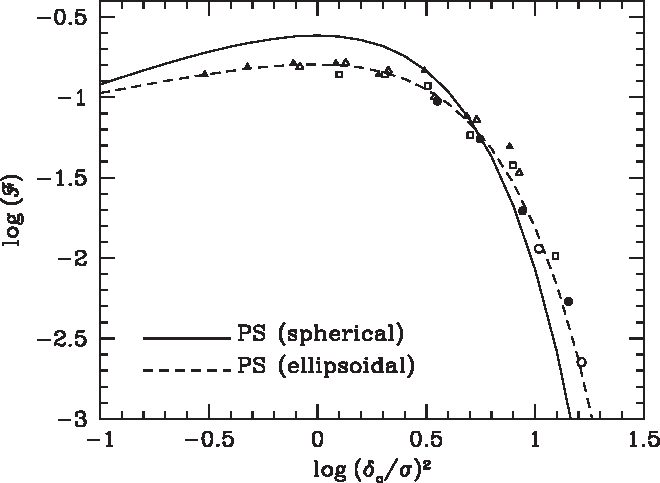
\includegraphics[width=\textwidth]{img/ch-04/PS.pdf}
	\caption{The multiplicity factor.}
	\label{fig:multiplicity}
\end{marginfigure}
\begin{marginfigure}
	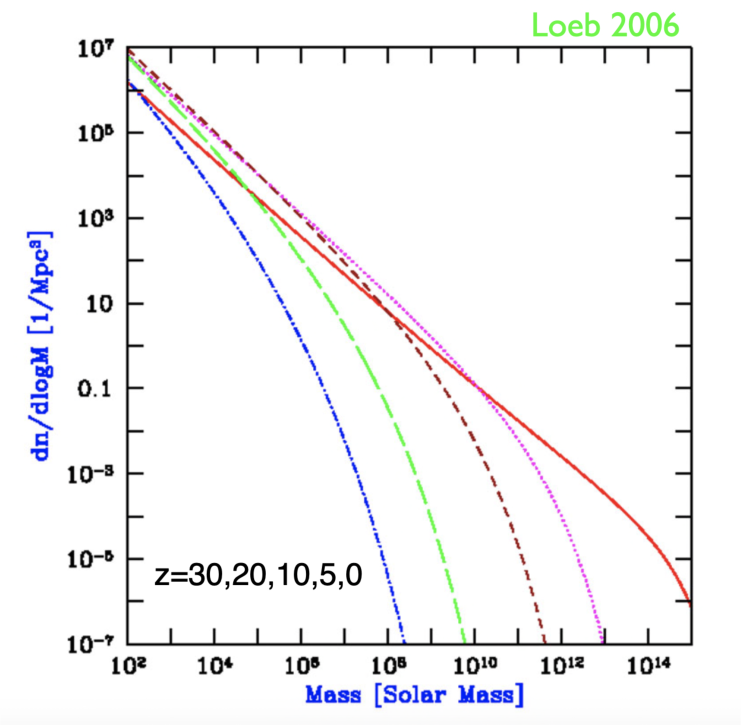
\includegraphics[width=\textwidth]{img/ch-04/dndm.pdf}
	\caption{The halo mass function.}
	\label{fig:dndm}
\end{marginfigure}


In \cref{fig:multiplicity}, we see that $f(\nu)$ from our model (solid line) corresponds acceptably to simulated data.
The agreement becomes much better when we allow elliptical collapse, which results in
\begin{align*}
	f_\text{EC}
	= A\left( 1 + \frac{1}{\tilde{\nu}^{2q}} \right) f_\text{PS}(\tilde{\nu}),
\end{align*}
where $\tilde{\nu} \approx 0.84 \nu$, $q = 0.3$, and $A \approx 0.322$.
There are also other fitting functions that are commonly used.


Let's look at the shape and evolution of the Mass function, shown in \cref{fig:dndm}.
The mass function is shown for different redshifts, where time increases from left to right.

The form of the mass function is $n \propto \nu \exp(-\nu^2/2)$, 
so there is an exponential cut-off for $\nu > 1$,
which we can see in the plot.
This corresponds to $M > M_*$, with $\sigma(M_*) = \delta_c(t)$.
Since in CDM models, $D(t)$ increases with $t$, and $\sigma(M)$ decreases with $M$,
$M_*$ increases with $t$.
This means that the cut-off occurs at higher masses as time goes on.
Thus, small haloes can form first, and massive haloes form later.
We have already seen this hierarchical structure formation before.


Today, the largest haloes which have formed have masses $M \approx \num{e14} M_\sol$.
At earlier epochs, the largest haloes were found in dwarf galaxies, with $M \approx \num{e9}$,
later galaxies with $M \approx \num{e12} M_\sol$,
and finally galaxy clusters with  $M \approx \num{e13} M_\sol$.




\section{Halo mergers}

We consider a halo with mass $M_0$ at time $t_0$.
A convenient description of the history of haloes are merger trees, such as the one in \cref{fig:tree}.

\begin{marginfigure}
	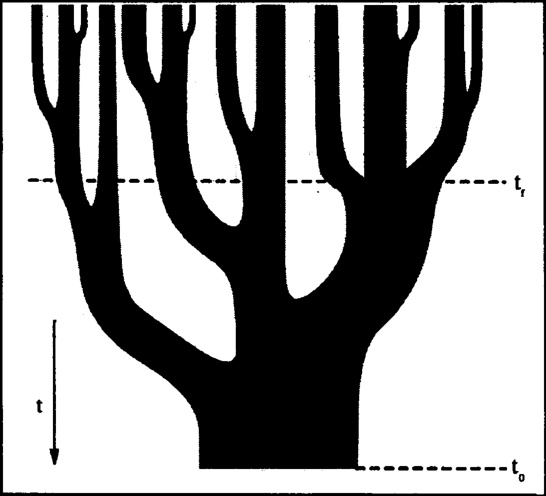
\includegraphics[width=\textwidth]{img/ch-04/tree.pdf}
	\caption{A merger tree represents the merging history of haloes. The thickness of a branch corresponds to its mass at that time. We see that several smaller progenitor haloes merge into more massive ones as time goes on.}
	\label{fig:tree}
\end{marginfigure}

Merger trees can be generated from numerical simulations, but the method is slow and not easy to understand intuitively.
Fortunately, an analytical approach, known as the \emph{extended Press-Schechter} (EPS) approach, exists.

\paragraph*{Progenitor mass function.}
Consider the average number of progenitors at time $t_1$ with masses $M_1 \in [M, M + \dd{M}]$, which by time $t_2$ have merged to form a halo of mass $M_2$.
\begin{align*}
	n(M_1, t_1 \, | \, M_2, t_2) \dd{M_1}
	&= \frac{M_2}{M_1} f_\text{PS}(\nu_{12}) \abs*{\dv{\ln \nu_{12}}{\ln M_1}} \dd{M_1},
\end{align*}
with
\begin{align*}
	\nu_{12}
	&= \frac{\delta_c(t_1) - \delta_c(t_2)}{\sqrt{\sigma^2(M_1) - \sigma^2(M_2)}}.
\end{align*}
This can be derived using the \textsc{eps} formalism.

\paragraph*{Main progenitor.}
The most massive branch of a merger tree is called the main progenitor.
In \cref{fig:progenitor-sample}, a sample of main progenitor histories for a given mass is shown, and in \cref{fig:progenitor-average}, averages of such histories for various masses are shown.

\begin{marginfigure}
	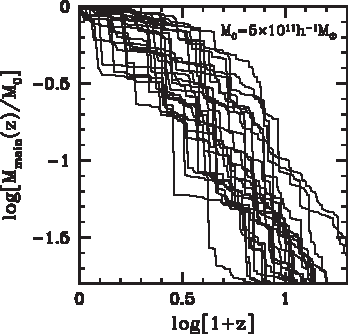
\includegraphics[width=\textwidth]{img/ch-04/progenitor-sample.pdf}
	\caption{A sample of progenitor histories with mass $M_0 = \num{5e11} h^{-1} M_\sol$.
	Each line shows the evolution of the mass of the main progenitor for a different halo.
	Note that there is a large scatter in the history of the main progenitors.}
	\label{fig:progenitor-sample}
\end{marginfigure}

\begin{marginfigure}
	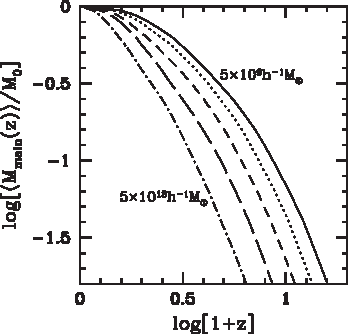
\includegraphics[width=\textwidth]{img/ch-04/progenitor-average.pdf}
	\caption{The average main progenitor histories of mergers with various masses. Each line is the average of many main progenitors with the same mass. We can see that massive haloes assemble quicker, but later}
	\label{fig:progenitor-average}
\end{marginfigure}



\paragraph*{Characteristic scales}

The \emph{assembly time} $t_a$ is the characteristic time scale for the formation of the halo.
It is defined such that the mass of the main progenitor at $t_a$ is half the final mass.

The \emph{halo merger rate} is the rate at which a halo of mass $M$ changes its mass by $\Delta M$, which can be expressed as a probability $\Prob(\Delta M \, | \, M, t) \dd{\ln \Delta M} \dd{\ln t}$.

The \emph{halo survival time} $t_s$ is the time it takes a halo of mass $M$ to merge to a halo of mass $2 M$.






\section{Halo clustering}


We want to study how haloes are clustered in space.
Consider the number overdensity of halos,
\begin{align*}
	\delta_h(\vec{x}, t)
	&= \frac{N_h - \bar{N}_h}{\bar{N}_h},
\end{align*}
where $N_h$ is the number of haloes with mass in $[M, M + \dd{M}]$ in a small volume $\dd{V}$ centred on position $\vec{x}$, 
and $\bar{N}_h$ is the mean number of such haloes.

\subsection{Linear Halo bias}
On linear (large) scales, one can show with the EPS-approach that
\begin{align*}
	\delta_h(\vec{x}, t)
	&= b_h(M, t) \delta(\vec{x}, t),
\end{align*}
where $b_h$ is a constant, called the \emph{halo bias},
and $\delta$ is the matter overdensity.
The halo bias can be derived to be
\begin{align*}
	b_h(M, t)
	= 1 + \frac{1}{D(t)}
	\left[ \frac{\nu^2 -1}{\delta_c(t)} \right],
\end{align*}
where we remember $\nu = \delta_c(t) / \sigma(M)$.

\begin{marginfigure}
	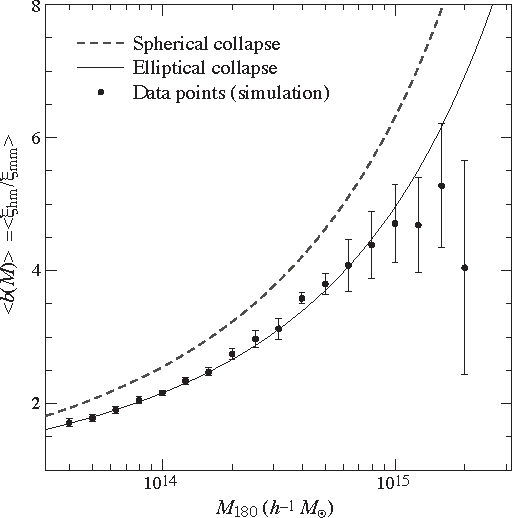
\includegraphics[width=\textwidth]{img/ch-04/halo-bias.pdf}
	\caption{The average bias for halos of mass $> M_{180}$ predicted by analytical models of spherical and elliptical collapse.}
	\label{fig:halo-bias}
\end{marginfigure}

The model is compared with simulations in \cref{fig:halo-bias}.
The dashed line is the spherical-collapse EPS model, and the solid line is a model that also includes non-spherical collapse.
Once again, we see that spherical collapse gives us the right trend, but introducing elliptical collapse yields a much better agreement with simulations.

% TODO? figure other fitting functions   Seljak & Warren 2004
Note that for $M > \num{1e12} M_\sol$, the halo bias is larger than $1$, so haloes are more clustered than $\delta$.
For $M < \num{1e12} M_\sol$ (not shown in the figure), $b_h < 1$, which is called an antibias.
In summary, the more massive the haloes, the more strongly clustered they are.

\subsection{More general bias models}

\paragraph*{Small scales.}
On small scales, we have to include non-linear effects in the bias.
Also, there could be a stochastic component to the bias.
Consider a more general bias model:
\begin{align*}
	\delta_h(\vec{x}, t)
	&= 
	b_h(M, t, \delta) \delta(\vec{x})
	+ \epsilon(\vec{x}) 
\end{align*}
where $b_h(\dots, \delta)$ leads to non-linear dependence on the bias, and $\epsilon$ describes the scatter between the halo contrast and the density contrast.

\paragraph*{Assembly bias.}
The bias may also depend on other halo properties, such as the concentration of the halo or its spin.
An important dependence is on the halo formation history.
It is found that haloes with early assembly times are more strongly clustered at a given mass and time. This is called \emph{assembly bias}.





\section{Internal structure of Haloes}

\subsection{Density profile}
From simulations, we know that density profiles of haloes are well fit by an NFW model (see \cref{ssec:spherical-models}),
\begin{align*}
	\rho(r)
	= \frac{\rho_s}{\left( \frac{r}{r_s} \right) \left( 1 + \frac{r}{r_s} \right)^2},
\end{align*}
where $\rho_s$ and $r_s$ are constants.
Note that the NFW profile is one of the double power law models.
We see that
\begin{align*}
	\rho(r)
	\propto
	\begin{cases}
		r^{-1} & \text{if } r \ll r_s\\
		r^{-2} & \text{if } r \approx r_s\\
		r^{-3} & \text{if } r \gg r_s,
	\end{cases}
\end{align*}
which is similar to the singular isothermal sphere model.
Since the model becomes invalid for $r \to 0$ because of the influence of baryons, the singularity at $r = 0$ is not a huge problem.
The total mass is
\begin{align*}
	M
	&= \int_0^{r_v} \dd{^3\vec{x}} \rho(\vec{x})\\
	&= 4\pi \int_0^{r_v} \dd{r} r^2 \rho(r)\\
	&= 4\pi \rho_s r_s^3 \left[ \ln(1+x) - \frac{c}{1+c} \right],
\end{align*}
where $r_v$ is the virial radius, defined such that $\rho(< r_v)/\bar{\rho} = 1 + \Delta_v \approx 178$ in a matter dominated universe.
The parameter $c = r_v/r_s$ is the concentration parameter.

Notes:
\begin{itemize}
	\item Sometimes, $\Delta_v = 200$ is approximated as a convention.
	\item The NFW profile is a good fit to haloes for all masses and redshifts in simulations, which is why it is called a \emph{universal profile}.
	It is not well-understood why there is such little variety in the large-scale structure of haloes.
	\item Generally, the concentration parameter $c(M, t)$ depends on mass and time.
	The dependence can be derived from simulations, but has so far not been predicted from analytical models.
	\item To a lesser degree, $c$ also depends on the formation history of the haloes, as haloes with early assembly times are more concentrated.
	\item There is an even better popular fit function, called the Einasto profile.
	It is flatter as $r \to 0$, but it also has more parameters.
\end{itemize}




\subsection{Shape}
Generally, haloes are not spherical, but elliptical.
Let $a_1 \geq a_2 \geq a_3$ be the main axes of the ellipsoid, and let $s = a_3/a_1$, which is a measure of flattening of the halo.

If $s = 1$, we are looking at a sphere, and $s=0$ is a perfectly flat two-dimensional pancake.
In simulations, the following trends have been found:
\begin{itemize}
	\item Less massive haloes are more spherical.
	\item Haloes that assemble early are more spherical.
	\item The minor axis $a_1$ tends to be perpendicular to large-scale filaments of the cosmic web.
\end{itemize}



\subsection{Substructure}

\begin{figure}
	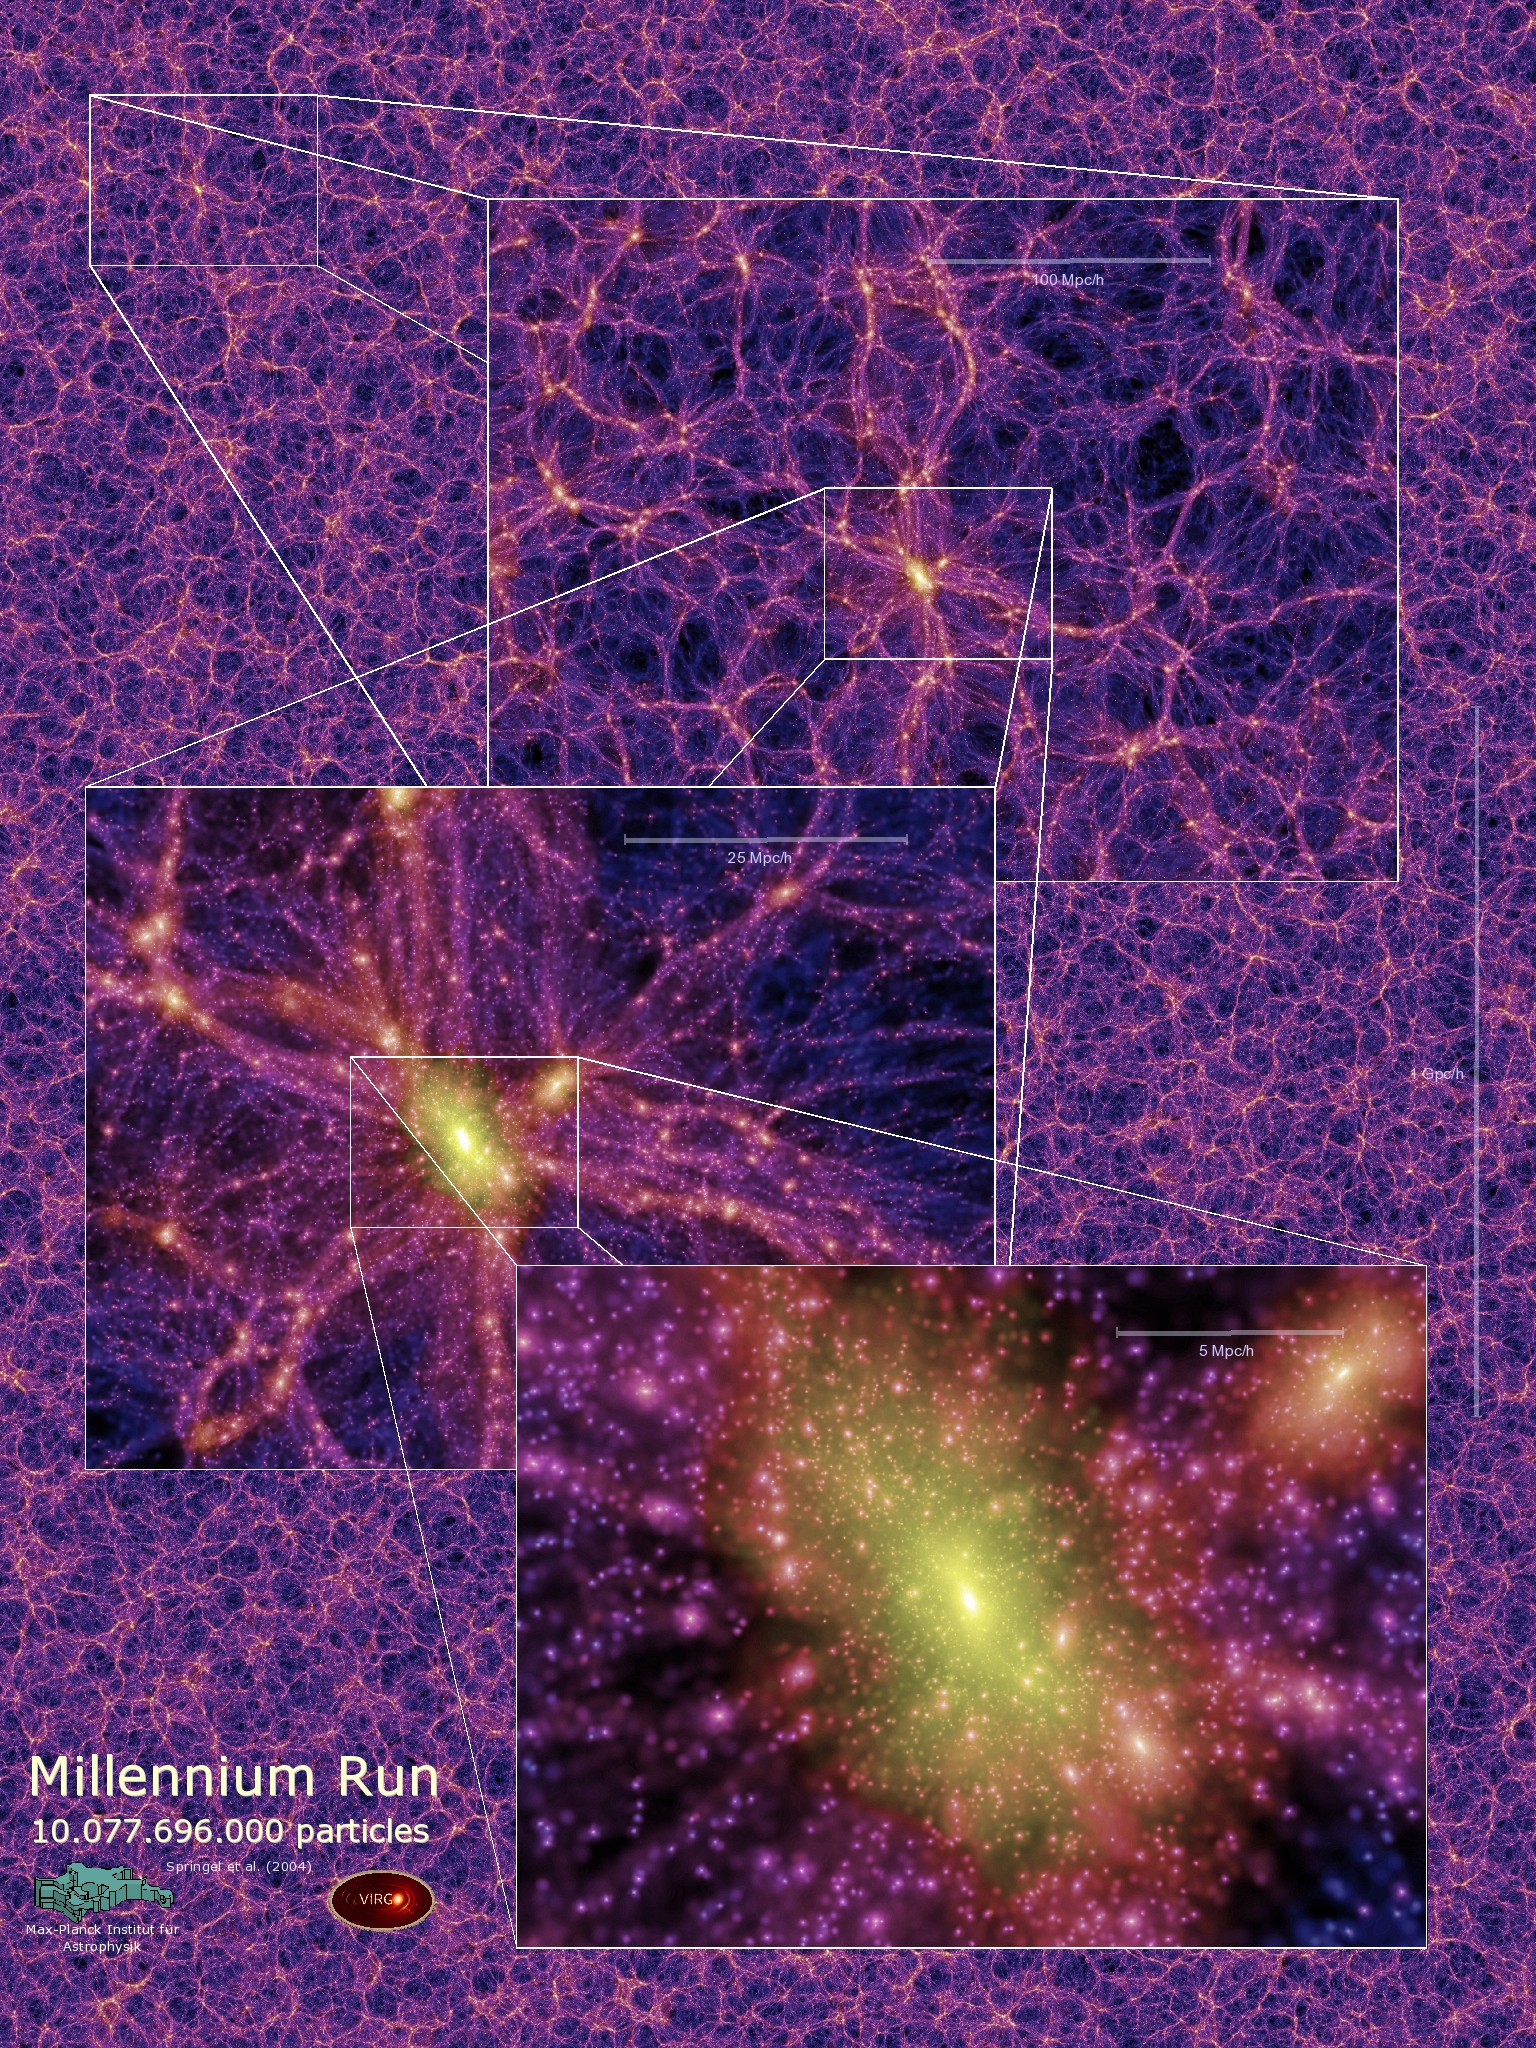
\includegraphics[width=\textwidth]{img/ch-04/millenium-run.png}
	\caption{The distribution of dark matter in the universe, based on the \enquote{Millenium Run} simulation. The halo in the enlarged view consists both of a smooth dark matter distribution and several smaller subhaloes. These subhaloes are remnants of progenitor haloes that have merged to form the main halo.}
	\label{fig:millenium-run}
\end{figure}

In \cref{fig:millenium-run}, we see the result of a large scale simulation of the universe.
In the dark matter distribution, there are subhaloes visible inside some haloes.
The subhaloes are remnants of progenitor haloes that have merged to form larger haloes.


An interesting quantity is the \emph{subhalo mass fraction}, which describes the number of subhaloes $n$ with mass $m$ in a main halo with total mass $M$.
To make the result independent of the mass of the main halo, we use the mass fraction $m/M$.

A good fit to simulations of the subhalo mass fraction is
\begin{align*}
	\dv{n}{\ln(m/M)}
	\approx 
	\frac{f_0}{\beta \Gamma(1-\gamma)}
	\left( \frac{m}{\beta M} \right)^{-\gamma}
	\exp\left( - \frac{m}{\beta M} \right),
\end{align*}
where $\gamma \approx 0.9$, $\beta \in [0.1, 0.5]$, and
\begin{align*}
	f_0
	= \frac{1}{M}
	\int m \dv{M}{m} \dd{m}.
\end{align*}
The quantity $f_0$ is called the \emph{mean subhalo mass fraction}, and it is the fraction of the main halo mass that is made up of subhaoles.

Subhaloes at a given time can be related to the progenitors and the survival time of progenitors following the merger.


\subsection{Angular momentum}
Haloes generally have a non-zero angular momentum, which can be characterized by the \emph{dimensionless spin parameter},
\begin{align*}
	\lambda = \frac{J \abs{E}^{1/2}}{G M^{5/2}},
\end{align*}
where $J$ is the angular momentum of the halo, $E$ is its energy, and $M$ is its mass.
From simulations, we know that $\lambda \approx 0.03$ is quite small, which is related to haloes being supported against gravitational collapse mostly by random motion rather than rotation.






